\chapter{Einleitung}


\section{Motivation}
In diesem Versuch beschäftigen wir uns mit verschiedenen Methoden der Temperaturmessung. Zunächst werden ein Gas- und ein Platin-Widerstandsthermometer im Bereich zwischen dem Siedepunkt von Wasser und dem Siedepunkt von flüssigem Stickstoff eingesetzt. Anschließend erfolgen Messungen im Bereich von 0 °C bis 100 °C mit einem Infrarot-Thermometer. Zuletzt wird mithilfe eines Thermoelements die Temperaturverteilung einer Bunsenbrennerflamme untersucht. Ziel des Versuchs ist es, die Ergebnisse der vier Methoden hinsichtlich ihrer Anwendbarkeit in verschiedenen Temperaturbereichen sowie ihrer Genauigkeit zu überprüfen.

\section{Physikalische Grundlagen}
\cite{skript25, demtroeder17}
\paragraph{Gasthermometer}
Die Grundlage bildet die ideale Gasgleichung
\begin{equation}
    pV = N k_{\mathrm{B}} T,
\end{equation}
wobei $p$ der Druck, $V$ das Volumen, $T$ die absolute Temperatur, $N$ die Teilchenzahl und $k_{\mathrm{B}}$ die Boltzmann-Konstante ist.  
Bei konstantem Volumen folgt das Gesetz von Amontons:
\begin{equation}
    T \propto p \quad (V = \text{konstant}).
\end{equation}
Das im Praktikum verwendete Gasthermometer besteht aus einem Glasballon, der über eine Kapillare mit einem Manometer verbunden ist. Systematische Fehler entstehen durch die thermische Ausdehnung des Ballons und durch das „schädliche Volumen“ der Luftsäule in der Kapillare, die bei Raumtemperatur bleibt. Diese Effekte sind jedoch klein gegenüber der Temperaturabhängigkeit des Drucks. Luft kann oberhalb des Verflüssigungspunktes und bei niedrigem Druck als ideales Gas angenähert werden.  

Zur Korrektur realer Gase könnte die van-der-Waals-Gleichung verwendet werden:
\begin{equation}
    \left(p + \frac{n^2 a}{V^2}\right)(V - nb) = nRT,
\end{equation}
mit den Stoffmengen $n$, der Gaskonstante $R$ sowie den stoffabhängigen Konstanten $a$ und $b$.

\paragraph{Thermoelement}
Die Funktionsweise beruht auf dem Seebeck-Effekt: An der Kontaktstelle zweier unterschiedlicher Metalle entsteht eine Thermospannung
\begin{equation}
    U_{\mathrm{th}} = K \, (T_1 - T_2),
\end{equation}
wobei $T_1$ die Temperatur an der Kontaktstelle, $T_2$ die Referenztemperatur und $K$ eine materialabhängige Konstante ist.  
Vorteile: kleiner Messfühler, große Temperaturbereiche, robuste Bauweise, geringe Kosten.  
Nachteil: Nur relative Messungen möglich, die Referenztemperatur $T_2$ muss bekannt oder konstant sein. Für präzise Messungen wird eine definierte Vergleichsstelle benötigt.  

\paragraph{Platin-Widerstandsthermometer}
Die Temperaturabhängigkeit des Widerstands eines Pt100-Sensors lässt sich durch ein quadratisches Polynom annähern:

\begin{equation}
    R(T) = R_0 \,(1 + A T + B T^2),
    \label{eq:r_von_t}
\end{equation}

mit dem Nennwiderstand $R_0 = 100\,\Omega$ bei $0^\circ$C und den Koeffizienten 
\begin{align}
    A &= 3,9083 \cdot 10^{-3}\,\mathrm{^\circ C^{-1}} \\
    B &= -5,775 \cdot 10^{-7}\,\mathrm{^\circ C^{-2}}
\end{align}

Ergibt sich eine Gleichung zur Berechnung der Temperatur $T$ in Anhänigkeit des Widerstandes $R$:

\begin{equation}
    T(R) = \frac{-R_0A + \sqrt{R_0^2 A^2 - 4 R_0 B (R_0 - R)}}{2 R_0 B}.
    \label{eq:t_pt100}
\end{equation}
Der Temperaturfehler für ein Pt100 der Klasse B beträgt

\begin{equation}
    \Delta T = 0{,}30\,^\circ\mathrm{C} + 0{,}005 \cdot |T|.
\end{equation}
Die Widerstandsmessung erfolgt im Praktikum mit einer Konstantstromquelle von $1\,$mA. Um Leitungseinflüsse zu vermeiden, wird eine Vierleiterschaltung verwendet.

\begin{figure}[h!]
    \centering
    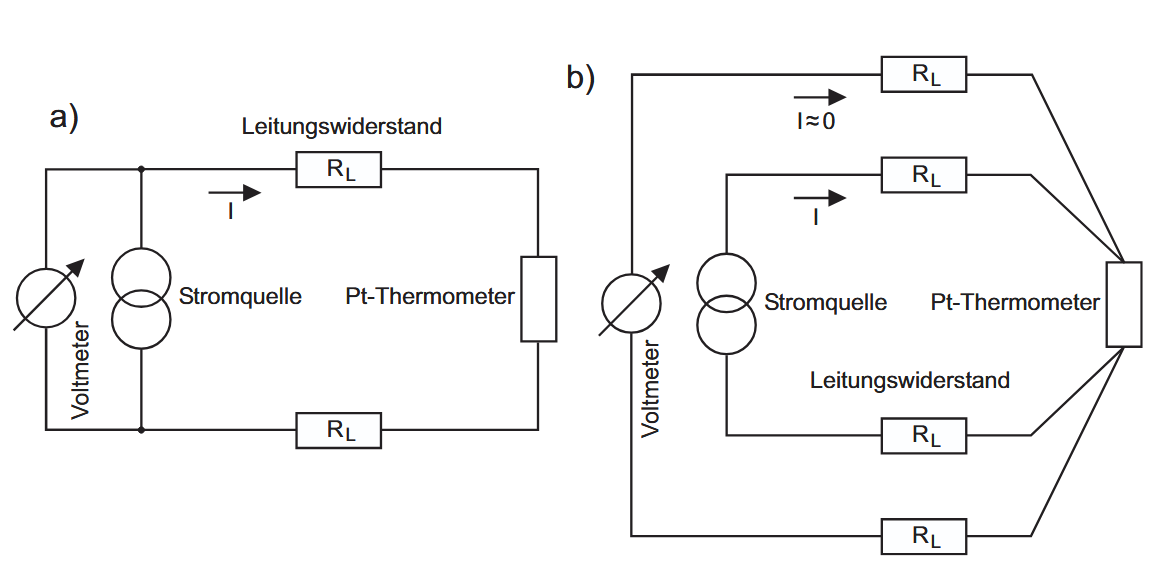
\includegraphics[width=0.45\textwidth]{img/41/zwei_vier-Leiter.png}
    \caption{Schematicher Aufbau einer a) Zweileiterschaltung und b) einer Vierleiterschaltung.}
\end{figure}

\paragraph{Pyrometer}
Jeder Körper mit $T > 0\,$K emittiert Wärmestrahlung. Das Plancksche Strahlungsgesetz beschreibt die spektrale Strahlungsleistung:
\begin{equation}
    M_\lambda(\lambda,T)\,dA\,d\lambda = \frac{2\pi h c^2}{\lambda^5} \cdot \frac{1}{e^{hc/(\lambda k_{\mathrm{B}}T)} - 1} \, dA\,d\lambda,
\end{equation}
wobei $h$ das Plancksche Wirkungsquantum und $c$ die Lichtgeschwindigkeit ist.  

Die gesamte abgestrahlte Leistung eines Körpers folgt aus dem Stefan-Boltzmann-Gesetz:
\begin{equation}
    P = \epsilon(T) \sigma A T^4,
\end{equation}
mit $\sigma$ als Stefan-Boltzmann-Konstante und dem Emissionsfaktor $\epsilon(T) \leq 1$.  
Das eingesetzte IR-Pyrometer misst im Bereich von $8$ bis $14\,\mu$m. Bei Raumtemperatur ($T \approx 300\,$K) liegt das Strahlungsmaximum bei $\lambda \approx 10\,\mu$m.

\section{Versuchsaufbau}
    
\begin{figure}[h!]
    \centering
    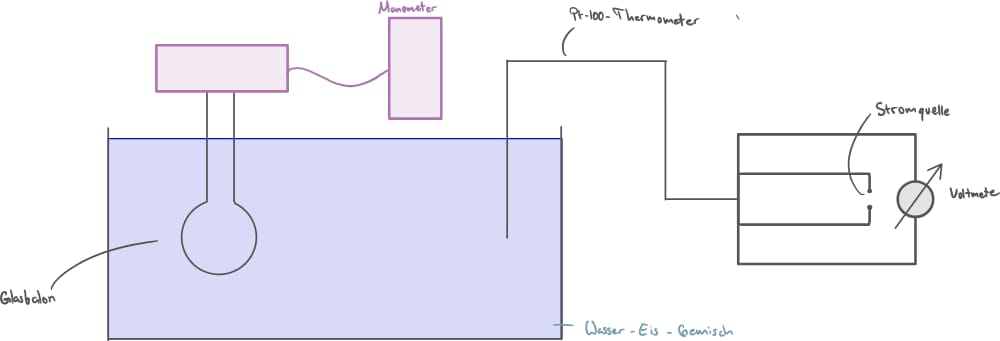
\includegraphics[width=0.4\textwidth]{img/41/1.jpg}
    \caption{Versuchsaufbau Eichung bei $0^\circ C$ mit Vierteiler Schaltung.}
\end{figure}

\begin{figure}[h!]
    \centering
    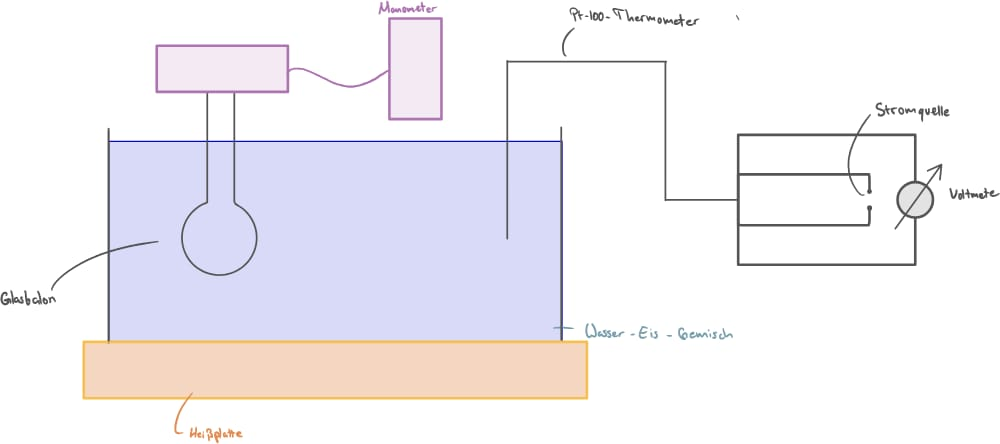
\includegraphics[width=0.4\textwidth]{img/41/2.jpg}
    \caption{Versuchsaufbau Temperaturmessung bis $100^\circ C$ mit Vierteiler Schaltung.}
\end{figure}

\begin{figure}[h!]
    \centering
    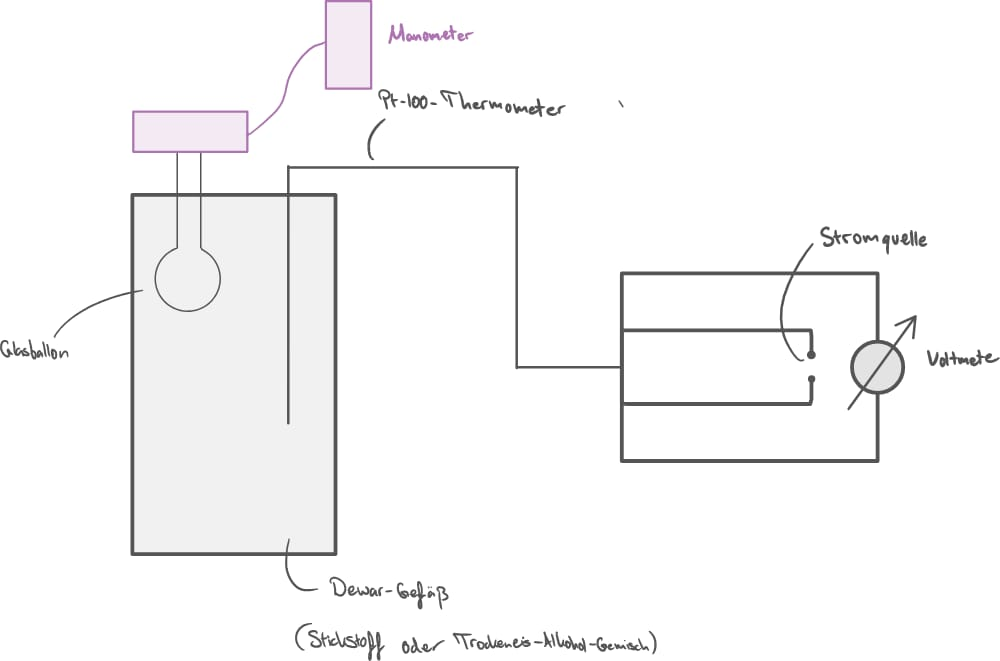
\includegraphics[width=0.3\textwidth]{img/41/3.jpg}
    \caption{Druck- und Spannungsmessung von Trockeneis-Alkohol-Gemisch und Flüssigstickstoff.}
\end{figure}

